\section{Visione generale delle strategie di verifica}
\subsection{Obiettivi di qualità}
	Per garantire la qualità del prodotto e dei processi utilizzati per realizzarlo il team Ottobit si è proposto di fissare degli obiettivi da perseguire per tutta la durata del progetto.
	\subsubsection{Qualità dei processi}
	Per il conseguimento degli obiettivi riguardanti la qualità dei processi è stato deciso di adottare lo standard ISO/IEC 15504$^*$ anche detta SPICE acronimo di Software Process Improvement and Capability Determination. Questo standard viene utilizzato per eseguire una valutazione concreta della qualità dei processi, inoltre permette la misurazione della capability$^*$ dei processi. All'\S\ appendice A è presente una descrizione delle caratteristiche dello standard.
	\subsubsection{Qualità del prodotto}
		Per quanto riguarda la qualità del prodotto si è scelto, in comune accordo, di seguire una serie di normative facenti parte dello standard ISO/IEC 9126$^*$, che definisce un modello dei requisiti qualitativi del Prodotto. Un completo approfondimento sullo standard ISO/IEC 9126 si trova in \S\ Appendice B.
\subsection{Organizzazione}
Per fare in modo che la qualità del prodotto finale rimanga entro i livelli prestabiliti, è necessario che ogni processo del progetto sia verificato prima di passare al successivo, al fine di intercettare eventuali errori ed evitarne la loro propagazione. Per essere certi di attuare la verifica nel modo corretto, i membri del gruppo dovranno attenersi ai principi definiti dagli standard scelti. In caso di perplessità potranno essere consultate le appendici di questo documento, dove vengono illustrati gli standard da rispettare per perseguire la qualità dei processi e del prodotto.

\subsection{Pianificazione strategica}
La strategia generale adottata è quella di automatizzare il più possibile le operazioni di verifica grazie all'utilizzo di strumenti volti allo scopo. L'obiettivo è avere un riscontro affidabile e misurabile che permetta di assicurare il grado di qualità stabilito precedentemente.  L'aspettativa è la riduzione del lavoro manuale permettendo così un'attività di verifica più semplice ed efficace.

\subsection{Responsabilità}
Il Verificatore ha il compito accertare che ogni modifica al materiale che costituisce il prodotto (codice, documentazione), effettuate dalle altre figure, venga svolta nella maniera corretta e nel rispetto delle regole definite in questo documento. Il Responsabile di progetto ha il compito di coordinare tutte le attività di verifica e di fare da garante della corretta esecuzione di tali, al fine di mantenere la qualità del materiale prodotto durante il suo ciclo di vita. Una descrizione più approfondita dei ruoli di progetto è inclusa nel documento  \textit{Piano di progetto}.

\subsection{Risorse}
Per svolgere queste operazioni il verificatore usufruirà di alcune risorse. Principalmente queste si dividono in due tipologie, le risorse necessarie sono quelle indispensabili per compiere il lavoro di verifica, quelle disponibili sono risorse alle quali il verificatore può attingere per eseguire il suo compito in modo efficacie ed efficiente.

\subsubsection{Necessarie}
I risultati del lavoro del gruppo devono essere disponibili a chiunque si occupi della verifica. Dunque i documenti o i files prodotti devono essere accessibili dal verificatore. Quest'ultimo dovrà disporre anche di un sistema per comunicare il risultato della verifica e i conseguenti problemi e cambiamenti da apportare, in modo che chi dovere posa porre rimedio alle mancanze nel più breve tempo possibile.

\subsubsection{Disponibili}
Il verificatore avrà a disposizione diversi strumenti per ottimizzare il processo di verifica e di valutazione. I documenti saranno fruibili dalla repository condivisa tra i membri del gruppo attraverso la piattaforma GitLab$^*$. I verificatori utilizzeranno un calcolatore di indice di Gulpease$^*$ e gli strumenti forniti dall'editor Latex$^*$ per notare meglio errori ortografici. Per notificare l'esito della verifica il verificatore potrà avvalersi di GitLab, del gruppo su Slack$^*$ oltre alla tabella di resoconto nella sezione §4 del \textit{Piano di qualifica}.

\subsection{Tecniche di verifica}
Per eseguire la verifica e la validazione potranno essere utilizzate tecniche di analisi statica o dinamica. Le prime sono le tecniche che si concentrano sullo studio della documentazione e del codice per accertarsi della presenza delle proprietà desiderate, l'assenza di difetti, e della conformità alle regole. A differenza di quelle statiche le tecniche di analisi dinamica richiedono l'esecuzione del codice e la verifica viene effettuata tramite prove del prodotto.\\
L'applicazione pratica delle tecniche di seguito presentate viene trattata nelle \textit{Norme di progetto}, affinché i membri del gruppo possano sempre avere un riferimento comune sulla verifica della qualità.
\subsubsection{Analisi statica}
Per la verifica della documentazione dovranno essere analizzate la correttezza grammaticale e ortografica, la correttezza degli argomenti trattati, la struttura del documento. Verranno utilizzati a questo scopo i correttori ortografici presenti negli editor Latex. Inoltre verrà calcolato l'indice di Gulpease per ogni documento redatto, grazie al quale sarà possibile valutare la complessità sintattica e la leggibilità del documento.\\
Per verificare il codice dell'applicazione che verrà creato sarà necessario analizzare diversi aspetti:
\begin{itemize}
\item Analisi del flusso di controllo: è necessaria per assicurarsi che il codice esegua nella sequenza desiderata e che esso sia ben strutturato. Non devono esistere parti di codice irraggiungibili o interminabili.
\item Analisi del flusso dei dati: controlla che non vengano utilizzate variabili senza che queste non siano state prima inizializzate. Non devono esistere variabili inutilizzate. 
\item Analisi del flusso di informazione: consiste nell'identificare le dipendenze tra informazioni passate in input e quelle prodotte in output dall’esecuzione di una unità di codice. Per assicurarsi che vengano rispettate le dipendenze previste e che non ci siano side effects indesiderati.
\end{itemize}
Questi tre aspetti potranno essere valutati grazie ad opportune misurazioni sulla complessità ciclomatica$^*$, numero di classi e coesione tra esse, complessità di flusso di informazioni.
\newpage
\subsubsection{Analisi dinamica}
L'analisi dinamica è il processo di valutazione$^*$ di un sistema software o di un suo componente, basato sull'osservazione del suo comportamento in esecuzione.
I componenti software che insieme formano il prodotto dovranno essere verificati attraverso diversi tipi di test, con lo scopo di garantire il corretto funzionamento dell'intero prodotto.
I test effettuati devono essere:
\begin{itemize}
\item misurabili e oggettivi;
\item ripetibili nel tempo, anche dopo una modifica al sistema;
\item eseguiti in una quantità sufficiente da provare la qualità del prodotto.
\end{itemize} 
Per la redazione dei test, il team ha deciso di seguire il V-Model$^*$ che descrive la relazione tra ogni fase del ciclo di vita dello sviluppo del software e la sua fase di testing.
\begin{figure}[htbp]
		\centering
		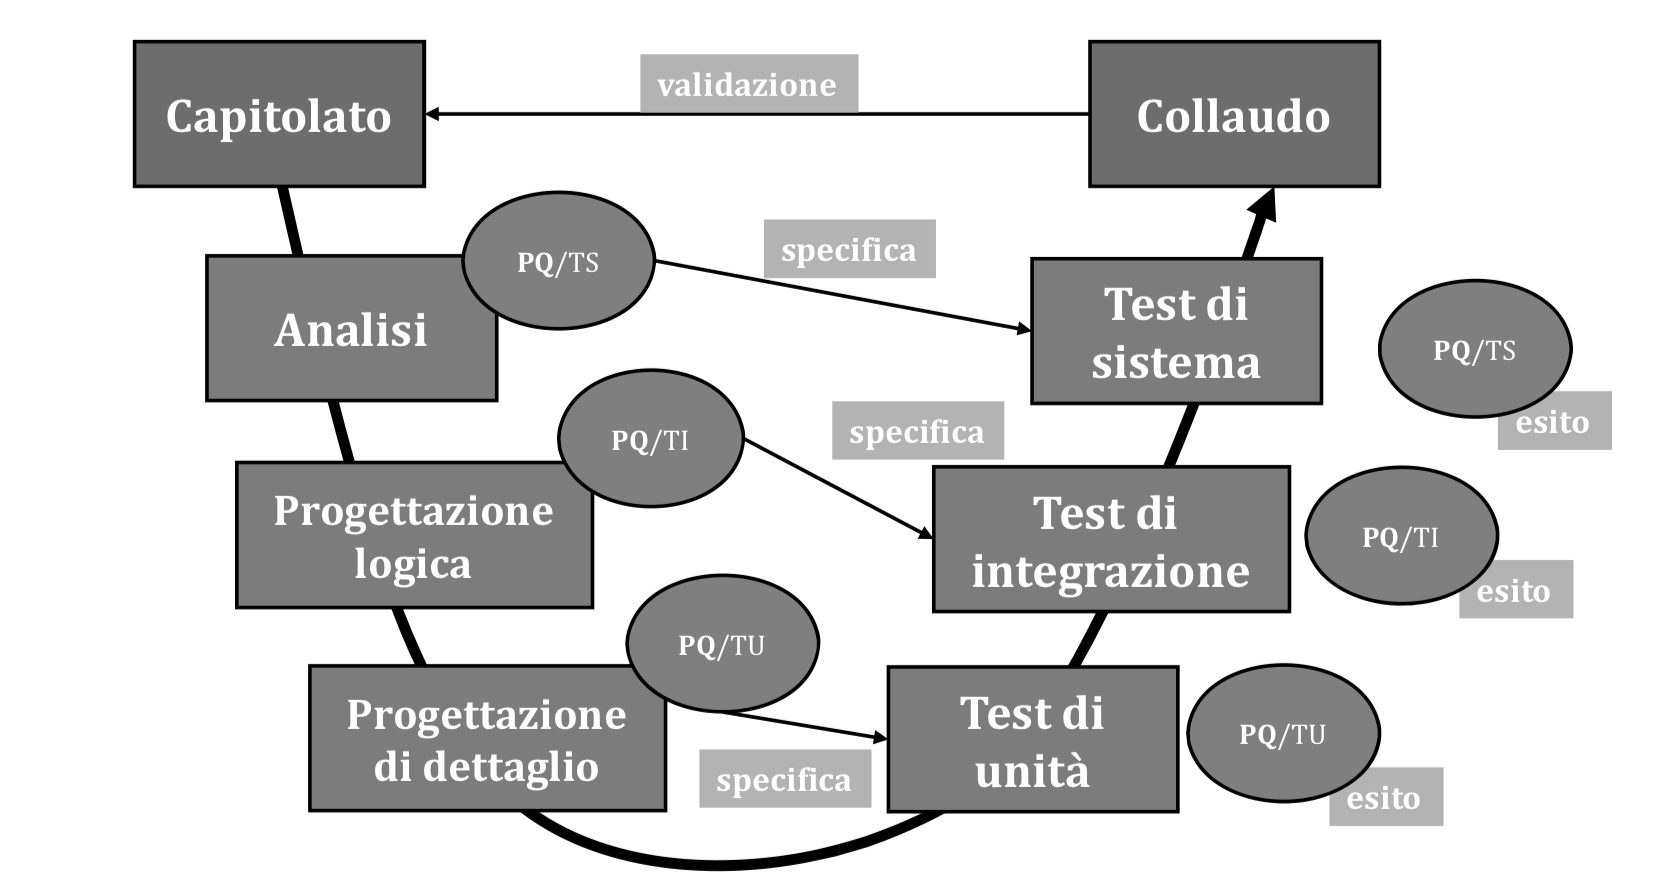
\includegraphics[scale=0.5]{images/vmodel.png}
		\caption{Rappresentazione del V-Model}
	
\end{figure}
\newline
Come descritto dal V-Model, i test vengono specificati e creati con l'avanzare del ciclo di vita del progetto, quindi verranno aggiunti all'interno di questo documento in maniera incrementale.
Le tipologie di test prese in considerazione sono:

\begin{itemize}
\item \textbf{Test di unità:} Consiste nella verifica di ogni singola unità del prodotto software. Per unità si intende la più piccola quantità di software che conviene verificare singolarmente.
\item \textbf{Test di integrazione:} Consiste nella verifica dell'insieme di due o più unità.
\item \textbf{Test di sistema:} Consiste nella verifica del sistema nel suo complesso, in modo da accertare la copertura dei requisiti.
\item \textbf{Test di regressione:} Consiste nell'eseguire nuovamente i test di unità, integrazione e sistema su componenti software che hanno subito delle modifiche, in modo da controllare che i cambiamenti apportati non abbiano pregiudicato il funzionamento.
\end{itemize}
